
In this chapter, we use the definition of the canonical ladder and the binary matrix representation of the canonical ladder to 
list $L_{n}$ in Gray code order. Recall, a Gray code is an ordering such that successive elements in the 
ordering differ 
by a minimal amount of change. When listing $L_{n}$, a minimal amount of change is defined as either adding or removing a bar, 
or relocating a bar; relocating a bar is the same as adding one bar and removing another. In the case of this chapter's 
algorithm, we add or remove a bar when transitioning between ladders in $L_{n}$. A key step in this chapter is that we are able to 
determine the bar corresponding to an inversion in constant time. Thus, the running time for this chapter's algorithm is CAT. 

\section{Equation: GetCoordinates2}
In the previous chapter, we described how 
we could list $L_{n}$ using the naive approach. However, using the naive approach is slow. In this chapter we seek to improve 
the running time for listing $L_{n}$. In this section, we improve the running time by determining the location of a bar in $O(1)$ time for a pair of adjacent elements. 
This allows us to take advantage of the Steinhaus-Johnson-Trotter algorithm, which applies adjacent transpositions to elements.\par  
We define $r$, with respect to a permutation $\pi$, as a vector of order $n$ as follows: $r_{x}$ equals the number of elements less than $x$ and to the 
right of $x$ in $\pi$. We note that $0 \leq r_{x} \leq x-1$. 
For example, given $(3,4,1,5,6,2)$, $r_{1}=0$, $r_{2}=0$, $r_{3}=2$, $r_{4}=2$, $r_{5}=1$ 
and $r_{6}=1$. We use $r$ to define {\sc GetCoordinates2} found in equation~\ref{Eqn:GetCoordinates2}. Let $x>y$ be two elements in $\pi$ 
such that $pos(x)=pos(y)+/-1$. We are going to apply an adjacent transposition to $x$ and $y$; we need to know where to 
locate the $1$ or $0$ in the binary matrix corresponding to the elements $x,y$ in order to flip it from a $1$ to a $0$ 
or vice versa. Prior to the transposition 
 of $x$ and $y$, if $pos(x) = pos(y)-1$ then {\sc GetCoordinates2} returns the row and column of the $1$ corresponding to $x$ and $y$.  
 If $pos(x)=pos(y)+1$, then {\sc GetCoordinates2} returns 
 the row and column of the $0$ corresponding to $x$ and $y$. $r_{x}$ is updated accordingly by being incremented or 
 decremented by $1$. 
 \begin{equation}\label{Eqn:GetCoordinates2}
    \resizebox{.9\textwidth}{!}{
      (row,column) = 
      \begin{cases}
        ((2n-x-1)-r_{x},(x-1)-r_{x}) & \text{ if pos(x)=pos(y)+1} \\ 
        ((2n-x)-r_{x},(x)-r_{x}) & \text{ if pos(y) = pos(x)+1}
      \end{cases}
    }
 \end{equation}

Initially, if $pos(x)=pos(y)+1$, then when we apply an adjacent transposition between $x$ and $y$, 
an inversion is induced in $\pi$. Therefore, $r_{x}$ is incremented by $1$, and the bar $(x,y)$ gets 
added to the canonical ladder. Initially, if $pos(x)=pos(y)-1$ then when we apply an adjacent 
transposition between $x$ and $y$, and an inversion gets removed from $\pi$. Therefore, $r_{x}$
is decremented by $1$, indicating the bar 
$(x,y)$ has been removed from the canonical ladder.
One of the main results of this thesis is {\sc ModifiedSJT} produces $L_{n}$ in Gray code order in CAT. 
{\sc ModifiedSJT} uses {\sc GetCoordinates2} and $r$ to calculate the row and column for every $1$ 
or $0$ in the binary matrix in $O(1)$ time.
%%section SJT

\section{Algorithm: ModifiedSJT}
In this section we define the algorithm {\sc ModifedSJT}, using $r$ and Equation~\ref{Eqn:GetCoordinates2}, 
which can be found in Algorithm~\ref{Alg:ModSJT}. Transposing two adjacent elements in $\pi_{i}$ results 
in a subsequent permutation $\pi_{j}$. The transposition of the two elements results in adding or removing a bar in 
$CL(\pi_{i})$, resulting in $CL(\pi_{j})$. The transposition of the two elements is merely simulated in Algorithm~\ref{Alg:ModSJT}, seeing 
as $\pi$ is not an argument to the function; we are able to calculate the location of the $1$ or $0$ in the binary matrix without 
having to induce the transposition in $\pi$. This makes our algorithm more interesting, seeing as we do not actually 
perform any swap operations on inversions. 
The initial conditions of {\sc ModifiedSJT} are the following:  
Let $ladder$ be the binary matrix representation of the canonical ladder such that 
each row and column coordinate along each associated diagonal is initialized to $0$.
Let $n$ be the maximum element.
Let $x$ be initialized to $2$; $x$ represents the current element. 
 On each recursive call 
$x$ is incremented by $1$ from $2,3 \dots n,n+1$. 
Let $direction$ be a one indexed array set to \textbf{false} for all indexes. $direction[x]=$\textsbf{false} implies the $xth$ element 
is being adjacently transposed 
from right to left. $direction[x]=$\textbf{true} implies the $xth$ element is being transposed from 
left to right. Let $r$ be the inversion vector initialized at all indices to $0$; when $r$ is initialized 
to all $0s$, this means that $r$ is the inversion vector for $\pi=(1,2, \dots, n-1,n)$.
\begin{algorithm}
  \begin{algorithmic}[1]
    \Function{ModifiedSJT}{$n$, $ladder$, $x$, $direction$, $r$}
     %%base case
      \If{$x > n$}
        \If{number of bars in $ladder$ equals $0$} {\sc Print}($ladder$)\EndIf
        \State \textbf{return}
      \EndIf
      %%swap the nth element n-1 times
      \For{$i$ \textbf{from} $1$ \textbf{to} $x$}
        \If{$i = 1$}
          \State {\sc ModifiedSJT}($n$, $ladder$, $x+1$, $direction$, $r$)
        \Else 
          \If{$direction[x]=$\textbf{false}}
            \State $(row,column) \gets ((2n-x-1)-r_{x},(x-1)-r_{x})$
            \State $r_{x} \gets r_{x}+1$ 
            \State $ladder[row][column] \gets 1$
          \Else
            \State $(row,column) \gets ((2n-x)-r_{x},(x)-r_{x})$
            \State $r_{x} \gets r_{x}-1$ 
            \State $ladder[row][column] \gets 0$
          \EndIf
          \State {\sc Print}($ladder$)
          \State {\sc ModifiedSJT}($n$, $ladder$, $x+1$, $direction$)
        \EndIf
        
      \EndFor
      \If{$direction[x] =$ \textbf{false}} $direction[x] \gets$ \textbf{true}
      \Else $\: direction[x] \gets$ \textbf{false}
      \EndIf
    \EndFunction
  \end{algorithmic}
  \caption{Modification of the {\sc SJT} algorithm for listing $L_{n}$}
  \label{Alg:ModSJT}
\end{algorithm}


\pagebreak

We use {\sc GetCoordinates2} on lines 10 and 14 of {\sc ModifiedSJT} to calculate the row and column. 
When $direction[x]$ equals \textbf{false} we use the first case from 
{\sc GetCoordinates2}. When $direction[x]$ equals \textbf{true} we use the second case from 
{\sc GetCoordinates2} to calculate the row and column.\par 

Given the current value of $x$, add or remove a bar for the route of $x$, then add or remove 
all bars for route $x+1$. Once all bars for route $x+1$ have been added or removed, 
proceed to add or remove the next bar from the route of $x$. Repeat until all $x-1$ bars have been added or removed from route $x$.
If $direction[x]$ is \textbf{false}, then bars of $x$ will be added to 
$ladder$ from right to left, bottom to top, until no more bars to the route of $x$ can be added.
If $direction[x]$ is \textbf{true}, then bars will be removed from $ladder$, left to right, top to bottom, until 
no more bars from the route of $x$ can be removed. Once all the bars for the route of $x$ have 
been added or removed, then $direction[x]$ is negated,
indicating that the opposite operation will be applied to the bars of the route of $x$ when 
$x$ is next processed. On each recursive call, $x$ is 
incremented by $1$. When $x$ is greater than $n$, return. 

\section{Analysis of {\sc ModifiedSJT}}
In this section we provide a theoretical analysis of {\sc ModifiedSJT} along with the runtime for the algorithm. 
We have implied that {\sc ModifiedSJT} produces $L_{n}$. 
We note that there are two general criteria for $L_{n}$. The first, each ladder in $L_{n}$ corresponds to a 
unique permutation of order $n$. The second, each ladder in $L_{n}$ is the canonical ladder. In Lemma~\ref{Lemma:ModSJTLn}, 
we prove the first criteria for $L_{n}$. 
\begin{lemma}
  Each ladder produced by {\sc ModifiedSJT} corresponds to a unique permutation of order $n$
  \label{Lemma:ModSJTLn}
\end{lemma}
\begin{proof}
  Since the algorithm is a modification of the Steinhaus-Johnson-Trotter algorithm, a similar proof for the SJT algorithm 
can be applied to the {\sc ModifiedSJT} algorithm. Suppose we want to list all $n!$ ladders 
of order $n$. Suppose we have all $n-1!$ ladders of order $n-1$, then for 
each ladder of order $n-1$ add a new column to the right; this results in $n-1$ columns seeing as 
the number of columns is one less than the number of elements. For each of the $n-1!$ ladders with $n-1$ columns 
add $0 \dots n-1$ bars beginning at column $n-1$ and ending 
at column $1$. Doing so results in $(n-1)!n=n!$ ladders of order $n$. To see 
an example of the proof please refer to Figure~\ref{Fig:CanLSJT}.
\end{proof}
%%prove the dimensions of the datastructure

\begin{center}
\begin{figure}[!htp]
  \centering
  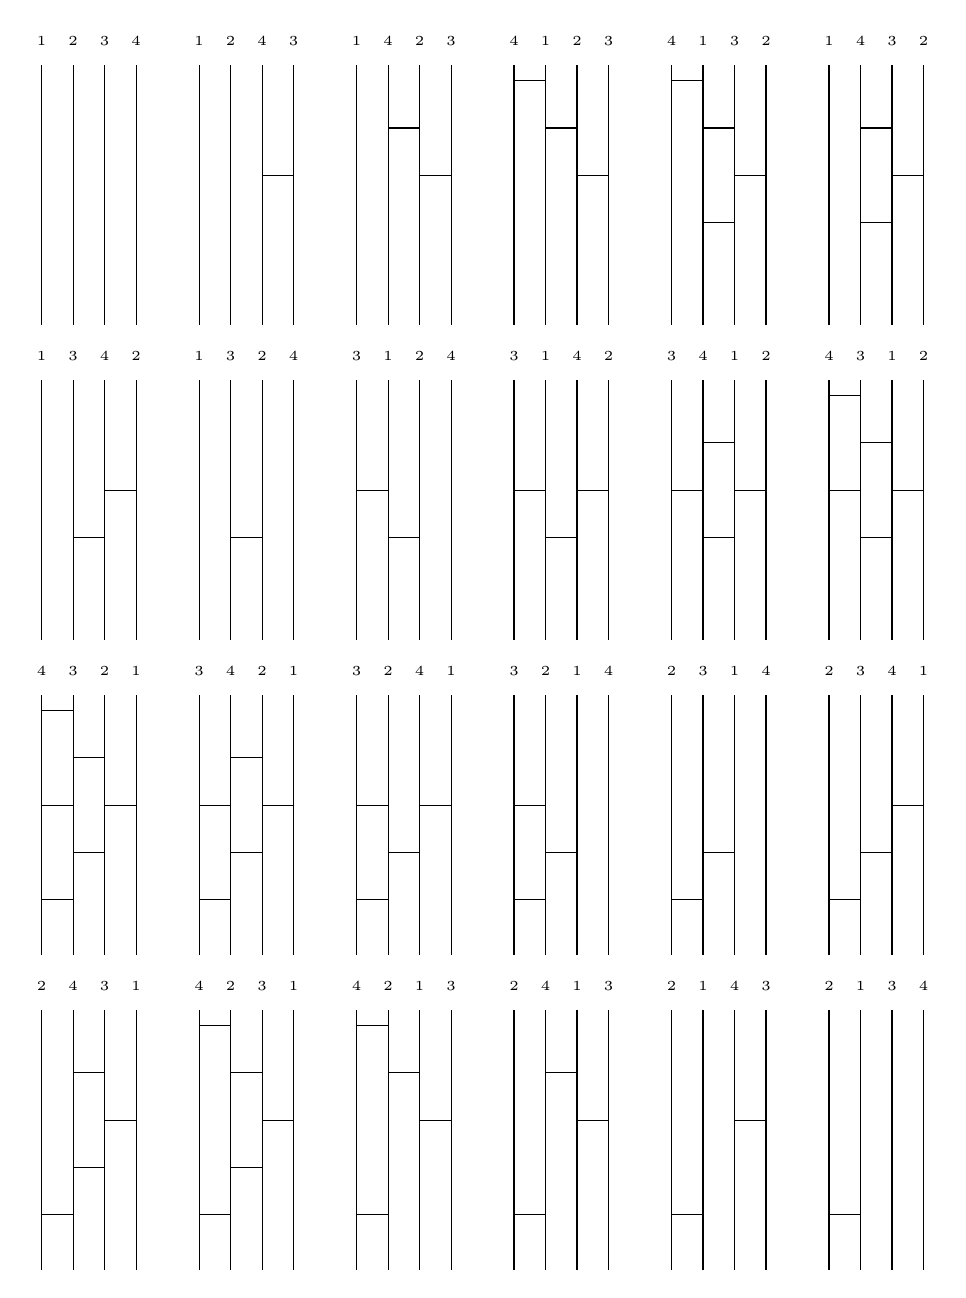
\begin{tikzpicture}

    \draw(0.00,9.70) to (0.00,13.00);
\draw(0.40,9.70) to (0.40,13.00);
\draw(0.80,9.70) to (0.80,13.00);
\draw(1.20,9.70) to (1.20,13.00);
\node at(0.00,13.30){\tiny{1}};
\node at(0.40,13.30){\tiny{2}};
\node at(0.80,13.30){\tiny{3}};
\node at(1.20,13.30){\tiny{4}};

\draw(2.00,9.70) to (2.00,13.00);
\draw(2.40,9.70) to (2.40,13.00);
\draw(2.80,9.70) to (2.80,13.00);
\draw(3.20,9.70) to (3.20,13.00);
\draw(2.80, 11.60) to (3.20, 11.60);
\node at(2.00,13.30){\tiny{1}};
\node at(2.40,13.30){\tiny{2}};
\node at(2.80,13.30){\tiny{4}};
\node at(3.20,13.30){\tiny{3}};

\draw(4.00,9.70) to (4.00,13.00);
\draw(4.40,9.70) to (4.40,13.00);
\draw(4.80,9.70) to (4.80,13.00);
\draw(5.20,9.70) to (5.20,13.00);
\draw(4.40, 12.20) to (4.80, 12.20);
\draw(4.80, 11.60) to (5.20, 11.60);
\node at(4.00,13.30){\tiny{1}};
\node at(4.40,13.30){\tiny{4}};
\node at(4.80,13.30){\tiny{2}};
\node at(5.20,13.30){\tiny{3}};

\draw(6.00,9.70) to (6.00,13.00);
\draw(6.40,9.70) to (6.40,13.00);
\draw(6.80,9.70) to (6.80,13.00);
\draw(7.20,9.70) to (7.20,13.00);
\draw(6.00, 12.80) to (6.40, 12.80);
\draw(6.40, 12.20) to (6.80, 12.20);
\draw(6.80, 11.60) to (7.20, 11.60);
\node at(6.00,13.30){\tiny{4}};
\node at(6.40,13.30){\tiny{1}};
\node at(6.80,13.30){\tiny{2}};
\node at(7.20,13.30){\tiny{3}};

\draw(8.00,9.70) to (8.00,13.00);
\draw(8.40,9.70) to (8.40,13.00);
\draw(8.80,9.70) to (8.80,13.00);
\draw(9.20,9.70) to (9.20,13.00);
\draw(8.00, 12.80) to (8.40, 12.80);
\draw(8.40, 12.20) to (8.80, 12.20);
\draw(8.80, 11.60) to (9.20, 11.60);
\draw(8.40, 11.00) to (8.80, 11.00);
\node at(8.00,13.30){\tiny{4}};
\node at(8.40,13.30){\tiny{1}};
\node at(8.80,13.30){\tiny{3}};
\node at(9.20,13.30){\tiny{2}};

\draw(10.00,9.70) to (10.00,13.00);
\draw(10.40,9.70) to (10.40,13.00);
\draw(10.80,9.70) to (10.80,13.00);
\draw(11.20,9.70) to (11.20,13.00);
\draw(10.40, 12.20) to (10.80, 12.20);
\draw(10.80, 11.60) to (11.20, 11.60);
\draw(10.40, 11.00) to (10.80, 11.00);
\node at(10.00,13.30){\tiny{1}};
\node at(10.40,13.30){\tiny{4}};
\node at(10.80,13.30){\tiny{3}};
\node at(11.20,13.30){\tiny{2}};

\draw(0.00,5.70) to (0.00,9.00);
\draw(0.40,5.70) to (0.40,9.00);
\draw(0.80,5.70) to (0.80,9.00);
\draw(1.20,5.70) to (1.20,9.00);
\draw(0.80, 7.60) to (1.20, 7.60);
\draw(0.40, 7.00) to (0.80, 7.00);
\node at(0.00,9.30){\tiny{1}};
\node at(0.40,9.30){\tiny{3}};
\node at(0.80,9.30){\tiny{4}};
\node at(1.20,9.30){\tiny{2}};

\draw(2.00,5.70) to (2.00,9.00);
\draw(2.40,5.70) to (2.40,9.00);
\draw(2.80,5.70) to (2.80,9.00);
\draw(3.20,5.70) to (3.20,9.00);
\draw(2.40, 7.00) to (2.80, 7.00);
\node at(2.00,9.30){\tiny{1}};
\node at(2.40,9.30){\tiny{3}};
\node at(2.80,9.30){\tiny{2}};
\node at(3.20,9.30){\tiny{4}};

\draw(4.00,5.70) to (4.00,9.00);
\draw(4.40,5.70) to (4.40,9.00);
\draw(4.80,5.70) to (4.80,9.00);
\draw(5.20,5.70) to (5.20,9.00);
\draw(4.00, 7.60) to (4.40, 7.60);
\draw(4.40, 7.00) to (4.80, 7.00);
\node at(4.00,9.30){\tiny{3}};
\node at(4.40,9.30){\tiny{1}};
\node at(4.80,9.30){\tiny{2}};
\node at(5.20,9.30){\tiny{4}};

\draw(6.00,5.70) to (6.00,9.00);
\draw(6.40,5.70) to (6.40,9.00);
\draw(6.80,5.70) to (6.80,9.00);
\draw(7.20,5.70) to (7.20,9.00);
\draw(6.00, 7.60) to (6.40, 7.60);
\draw(6.80, 7.60) to (7.20, 7.60);
\draw(6.40, 7.00) to (6.80, 7.00);
\node at(6.00,9.30){\tiny{3}};
\node at(6.40,9.30){\tiny{1}};
\node at(6.80,9.30){\tiny{4}};
\node at(7.20,9.30){\tiny{2}};

\draw(8.00,5.70) to (8.00,9.00);
\draw(8.40,5.70) to (8.40,9.00);
\draw(8.80,5.70) to (8.80,9.00);
\draw(9.20,5.70) to (9.20,9.00);
\draw(8.40, 8.20) to (8.80, 8.20);
\draw(8.00, 7.60) to (8.40, 7.60);
\draw(8.80, 7.60) to (9.20, 7.60);
\draw(8.40, 7.00) to (8.80, 7.00);
\node at(8.00,9.30){\tiny{3}};
\node at(8.40,9.30){\tiny{4}};
\node at(8.80,9.30){\tiny{1}};
\node at(9.20,9.30){\tiny{2}};

\draw(10.00,5.70) to (10.00,9.00);
\draw(10.40,5.70) to (10.40,9.00);
\draw(10.80,5.70) to (10.80,9.00);
\draw(11.20,5.70) to (11.20,9.00);
\draw(10.00, 8.80) to (10.40, 8.80);
\draw(10.40, 8.20) to (10.80, 8.20);
\draw(10.00, 7.60) to (10.40, 7.60);
\draw(10.80, 7.60) to (11.20, 7.60);
\draw(10.40, 7.00) to (10.80, 7.00);
\node at(10.00,9.30){\tiny{4}};
\node at(10.40,9.30){\tiny{3}};
\node at(10.80,9.30){\tiny{1}};
\node at(11.20,9.30){\tiny{2}};

\draw(0.00,1.70) to (0.00,5.00);
\draw(0.40,1.70) to (0.40,5.00);
\draw(0.80,1.70) to (0.80,5.00);
\draw(1.20,1.70) to (1.20,5.00);
\draw(0.00, 4.80) to (0.40, 4.80);
\draw(0.40, 4.20) to (0.80, 4.20);
\draw(0.00, 3.60) to (0.40, 3.60);
\draw(0.80, 3.60) to (1.20, 3.60);
\draw(0.40, 3.00) to (0.80, 3.00);
\draw(0.00, 2.40) to (0.40, 2.40);
\node at(0.00,5.30){\tiny{4}};
\node at(0.40,5.30){\tiny{3}};
\node at(0.80,5.30){\tiny{2}};
\node at(1.20,5.30){\tiny{1}};

\draw(2.00,1.70) to (2.00,5.00);
\draw(2.40,1.70) to (2.40,5.00);
\draw(2.80,1.70) to (2.80,5.00);
\draw(3.20,1.70) to (3.20,5.00);
\draw(2.40, 4.20) to (2.80, 4.20);
\draw(2.00, 3.60) to (2.40, 3.60);
\draw(2.80, 3.60) to (3.20, 3.60);
\draw(2.40, 3.00) to (2.80, 3.00);
\draw(2.00, 2.40) to (2.40, 2.40);
\node at(2.00,5.30){\tiny{3}};
\node at(2.40,5.30){\tiny{4}};
\node at(2.80,5.30){\tiny{2}};
\node at(3.20,5.30){\tiny{1}};

\draw(4.00,1.70) to (4.00,5.00);
\draw(4.40,1.70) to (4.40,5.00);
\draw(4.80,1.70) to (4.80,5.00);
\draw(5.20,1.70) to (5.20,5.00);
\draw(4.00, 3.60) to (4.40, 3.60);
\draw(4.80, 3.60) to (5.20, 3.60);
\draw(4.40, 3.00) to (4.80, 3.00);
\draw(4.00, 2.40) to (4.40, 2.40);
\node at(4.00,5.30){\tiny{3}};
\node at(4.40,5.30){\tiny{2}};
\node at(4.80,5.30){\tiny{4}};
\node at(5.20,5.30){\tiny{1}};

\draw(6.00,1.70) to (6.00,5.00);
\draw(6.40,1.70) to (6.40,5.00);
\draw(6.80,1.70) to (6.80,5.00);
\draw(7.20,1.70) to (7.20,5.00);
\draw(6.00, 3.60) to (6.40, 3.60);
\draw(6.40, 3.00) to (6.80, 3.00);
\draw(6.00, 2.40) to (6.40, 2.40);
\node at(6.00,5.30){\tiny{3}};
\node at(6.40,5.30){\tiny{2}};
\node at(6.80,5.30){\tiny{1}};
\node at(7.20,5.30){\tiny{4}};

\draw(8.00,1.70) to (8.00,5.00);
\draw(8.40,1.70) to (8.40,5.00);
\draw(8.80,1.70) to (8.80,5.00);
\draw(9.20,1.70) to (9.20,5.00);
\draw(8.40, 3.00) to (8.80, 3.00);
\draw(8.00, 2.40) to (8.40, 2.40);
\node at(8.00,5.30){\tiny{2}};
\node at(8.40,5.30){\tiny{3}};
\node at(8.80,5.30){\tiny{1}};
\node at(9.20,5.30){\tiny{4}};

\draw(10.00,1.70) to (10.00,5.00);
\draw(10.40,1.70) to (10.40,5.00);
\draw(10.80,1.70) to (10.80,5.00);
\draw(11.20,1.70) to (11.20,5.00);
\draw(10.80, 3.60) to (11.20, 3.60);
\draw(10.40, 3.00) to (10.80, 3.00);
\draw(10.00, 2.40) to (10.40, 2.40);
\node at(10.00,5.30){\tiny{2}};
\node at(10.40,5.30){\tiny{3}};
\node at(10.80,5.30){\tiny{4}};
\node at(11.20,5.30){\tiny{1}};

\draw(0.00,-2.30) to (0.00,1.00);
\draw(0.40,-2.30) to (0.40,1.00);
\draw(0.80,-2.30) to (0.80,1.00);
\draw(1.20,-2.30) to (1.20,1.00);
\draw(0.40, 0.20) to (0.80, 0.20);
\draw(0.80, -0.40) to (1.20, -0.40);
\draw(0.40, -1.00) to (0.80, -1.00);
\draw(0.00, -1.60) to (0.40, -1.60);
\node at(0.00,1.30){\tiny{2}};
\node at(0.40,1.30){\tiny{4}};
\node at(0.80,1.30){\tiny{3}};
\node at(1.20,1.30){\tiny{1}};

\draw(2.00,-2.30) to (2.00,1.00);
\draw(2.40,-2.30) to (2.40,1.00);
\draw(2.80,-2.30) to (2.80,1.00);
\draw(3.20,-2.30) to (3.20,1.00);
\draw(2.00, 0.80) to (2.40, 0.80);
\draw(2.40, 0.20) to (2.80, 0.20);
\draw(2.80, -0.40) to (3.20, -0.40);
\draw(2.40, -1.00) to (2.80, -1.00);
\draw(2.00, -1.60) to (2.40, -1.60);
\node at(2.00,1.30){\tiny{4}};
\node at(2.40,1.30){\tiny{2}};
\node at(2.80,1.30){\tiny{3}};
\node at(3.20,1.30){\tiny{1}};

\draw(4.00,-2.30) to (4.00,1.00);
\draw(4.40,-2.30) to (4.40,1.00);
\draw(4.80,-2.30) to (4.80,1.00);
\draw(5.20,-2.30) to (5.20,1.00);
\draw(4.00, 0.80) to (4.40, 0.80);
\draw(4.40, 0.20) to (4.80, 0.20);
\draw(4.80, -0.40) to (5.20, -0.40);
\draw(4.00, -1.60) to (4.40, -1.60);
\node at(4.00,1.30){\tiny{4}};
\node at(4.40,1.30){\tiny{2}};
\node at(4.80,1.30){\tiny{1}};
\node at(5.20,1.30){\tiny{3}};

\draw(6.00,-2.30) to (6.00,1.00);
\draw(6.40,-2.30) to (6.40,1.00);
\draw(6.80,-2.30) to (6.80,1.00);
\draw(7.20,-2.30) to (7.20,1.00);
\draw(6.40, 0.20) to (6.80, 0.20);
\draw(6.80, -0.40) to (7.20, -0.40);
\draw(6.00, -1.60) to (6.40, -1.60);
\node at(6.00,1.30){\tiny{2}};
\node at(6.40,1.30){\tiny{4}};
\node at(6.80,1.30){\tiny{1}};
\node at(7.20,1.30){\tiny{3}};

\draw(8.00,-2.30) to (8.00,1.00);
\draw(8.40,-2.30) to (8.40,1.00);
\draw(8.80,-2.30) to (8.80,1.00);
\draw(9.20,-2.30) to (9.20,1.00);
\draw(8.80, -0.40) to (9.20, -0.40);
\draw(8.00, -1.60) to (8.40, -1.60);
\node at(8.00,1.30){\tiny{2}};
\node at(8.40,1.30){\tiny{1}};
\node at(8.80,1.30){\tiny{4}};
\node at(9.20,1.30){\tiny{3}};

\draw(10.00,-2.30) to (10.00,1.00);
\draw(10.40,-2.30) to (10.40,1.00);
\draw(10.80,-2.30) to (10.80,1.00);
\draw(11.20,-2.30) to (11.20,1.00);
\draw(10.00, -1.60) to (10.40, -1.60);
\node at(10.00,1.30){\tiny{2}};
\node at(10.40,1.30){\tiny{1}};
\node at(10.80,1.30){\tiny{3}};
\node at(11.20,1.30){\tiny{4}};


    
    
    
  \end{tikzpicture}
  \caption{$L_{4}$ generated by the {\sc ModifiedSJT} algorithm. The algorithm inserts or removes a bar between any two successive ladders.}
  \label{Fig:CanLSJT}
\end{figure}
\end{center}
\pagebreak



%%end proof
To prove that each ladder produced by {\sc ModifiedSJT} is the canonical ladder, 
we prove that the calculations for the $(row,column)$ coordinates lie on the associated diagonal of $x$. 
Recall that the canonical ladder is the ladder such that for each element, $2 \leq x \leq n$, each  
bar associated with $x$ lies on the associated diagonal of $x$. The associated diagonal of $x$ starts at 
$(2n-2x+1, 1)$ and ends at $(2n-x-1, x-1)$. \par 
The calculations for the row and column for the bar 
depend on whether the bar is being added or removed. Thus, there are
four cases to consider. We will prove that for each case, the calculation for the $(row,column)$ coordinates is located 
along the associated diagonal of $x$. The cases are the following: 
\begin{caseof}
 ~\case{Bar is being added}{Row is being calculated.}
 ~\case{Bar is being added}{Column is being calculated.}
 ~\case{Bar is being removed}{Row is being calculated.}
 ~\case{Bar is being removed.}{Column is being calculated.}
\end{caseof}

%%End the cases

%%proof 1
\begin{lemma}
  Assume a bar is being added and a row is being calculated. 
  We use $(2n - x - 1) - r_{x}$ to calculate the row. The row calculation is bounded by the uppermost row and bottommost row composing the associated diagonal of $x$. 
  \label{Lemma:Case1}
\end{lemma}
\begin{proof}
   Suppose $r_{x}=0$, then we know that $x$ currently has no associated bars in the ladder. 
   We know that the first bar associated with $x$ will 
   be located at row $(2n-x-1)-0$ which is also the bottommost row composing the associated diagonal of $x$.  
   Suppose $r_{x}=x-2$, then we know that $x$ has one more associated bar be added to the ladder. The bar will be located at 
   $(2n - x - 1) - (x-2)$ which is simplified to $2n-2x+1$; $2n-2x+1$ equals the uppermost row composing the associated diagonal of $x$.  
\end{proof}

\begin{lemma}
  Assume a bar is being added and a column is being calculated. 
  We use $(x-1)-r_{x}$ to calculate the column. The column calculation is bounded by the leftmost column and rightmost column 
  composing the associated diagonal of $x$. 
  \label{Lemma:Case2}
\end{lemma}
\begin{proof}
  Suppose $r_{x}=0$, then we know that $x$ currently has no associated bars in the ladder. 
  We know that the first bar associated with $x$ will be located at $(x-1)-0$ which is also the rightmost column composing the associated 
  diagonal of $x$. Suppose $r_{x} = x-2$, then we know that $x$ has one more associated bar to be added to the ladder. The bar will 
  be located at $(x-1)-(x-2)$ which is simplified to $1$; $1$ equals the leftmost column composing the associated diagonal of $x$.

\end{proof}

\begin{lemma}
  Assume a bar is being removed and a row is being calculated. 
  We use $(2n - x)-r_{x}$ to calculate the row. The row is bounded by the uppermost row and bottommost row composing the 
  associated diagonal of $x$.
  \label{Lemma:Case3} 
  
\end{lemma}
\begin{proof}
  Suppose $r_{x}=x-1$, then we know that $x$ has all of its associated bars in the canonical ladder. We calculate the row of the first bar to 
  be removed at $(2n-x)-(x-1)=(2n - 2x)+1$; $(2n - 2x)+1$ is the uppermost row of the associated diagonal of $x$. Suppose $r_{x}=1$, then we know that 
  $x$ only has one more bar to be removed from the ladder. We calculate the row of the last bar to be removed at $(2n-x)-1$; $2n-x-1$ is the bottommost 
  row of the associated diagonal of $x$. 

\end{proof}
\begin{lemma}
  Assume a bar is being removed and a column is being calculated. We use $(x)-r_{x}$ to calculate the column. 
  The column is bounded by the leftmost column and rightmost column composing the associated diagonal of $x$.
  \label{Lemma:Case4}
\end{lemma}
\begin{proof}
  Suppose $r_{x}=x-1$, then we know that $x$ has all of its associated bars in the canonical ladder. We calculate the column 
  of the first bar to be removed at $(x)-(x-1)=1$; $1$ is the leftmost column of the associated diagonal of $x$. Suppose 
  $r_{x}=1$, then we know $x$ only has one more bar to be removed from the ladder. We calculate the column of the last bar to be 
  removed at $(x)-1$; $x-1$ is the rightmost column of the associated diagonal of $x$.
\end{proof}

Using Lemmas~\ref{Lemma:ModSJTLn},~\ref{Lemma:Case1},~\ref{Lemma:Case2},~\ref{Lemma:Case3},~\ref{Lemma:Case4} we have shown that 
{\sc ModifiedSJT} produces $L_{n}$. However, we have yet to prove that {\sc ModifedSJT} produces $L_{n}$ in Gray code order. 
We use Theorem~\ref{Theorem:GrayCoderOrderSJT} to prove that {\sc ModifiedSJT} produces $L_{n}$ in Gray code order. 
\begin{theorem}
  {\sc ModifiedSJT} produces $L_{n}$ in Gray code order
  \label{Theorem:GrayCoderOrderSJT}
\end{theorem}
\begin{proof}
  Let $l_{i}$ be an arbitrary ladder produced by {\sc ModifedSJT}. Let $j$ be the next ladder to be produced by {\sc ModifiedSJT}. If 
  $l_{i}=l_{j}$ plus or minus a bar, then {\sc ModifiedSJT} produces $L_{n}$ in Gray code order. On each iteration of the loop, $direction[x]$ 
  is either true or false, but not both. When $direction[x]=false$, a single $1$ is added to the associated diagonal of $x$, indicating 
  a bar has been added. When $direction[x]=true$, 
  a single $0$ is added to the associated diagonal of $x$, indicating a bar has been removed. With an addition or removal of a $1$ or $0$, $l_{i}$ 
  differs from $l_{j}$ by the addition or removal of a bar. Therefore, $L_{n}$ is produced by {\sc ModifedSJT} in Gray code order.
    
\end{proof}
\begin{theorem}
  {\sc ModifiedSJT} produces $L_{n}$ in CAT.
\end{theorem}
\begin{proof}
  The first ladder is printed in $O(n)$ time because $[2 \dots n+1]$ recursive calls are made 
before first ladder is printed. Each subsequent ladder deviates from its predecessor by a single addition or removal of a bar.
  Calculating the location of a $1$ or $0$, corresponding to a bar or absence of a bar, is done in $O(1)$ time. Once calculated, 
  the $1$ or $0$ is added to $l_{i}$ producing $l_{j}$. Once $l_{i}$ is transformed into $l_{j}$, $l_{j}$ is printed.
\end{proof}
We calculated the runtimes for $n=1 \dots 13$. The runtime is calculated without the ladders being printed.  
When the ladders are printed, the runtime increases by a substantial amount. 
The runtimes from $n=9 \dots n=13$ are provided in Table~\ref{Table:ListingResults}.
 \begin{center}
    \begin{table}[ht]
      \centering
      \caption{The table with the runtimes for listing $L_{n}$ using {\sc ModifiedSJT}.}

    \resizebox{.75\textwidth}{0.2\textheight}{
       \begin{tabular}{ |p{1cm}||p{5cm}|}
        \hline
        \multicolumn{2}{|c|}{Runtimes for generating $L_{n}$ in seconds} \\
        \hline
            $n$ & {\sc ModifiedSJT} Runtime\\
        \hline
            \small{9} &  \small{0.00}\\
            \hline 
            \small{10} &  \small{0.03}\\
            \hline
            \small{11} &  \small{0.25}\\
            \hline 
            \small{12} &  \small{2.78}\\
            \hline 
            \small{13} & \small{66.97}\\
        \hline
    \end{tabular}}
    \label{Table:ListingResults}
    \end{table}
  \end{center}


  \section{Chapter Conclusion}
  We have provided a CAT algorithm for listing $L_{n}$ by adding or removing a bar. By doing so, we 
  have provided a solution to The Canonical Ladder Listing Problem. We use Equation~\ref{Eqn:GetCoordinates2} and modified the 
  Steinhaus-Johnson-Trotter algorithm in order to create Algorithm~\ref{Alg:ModSJT}. We computed the location of a bar corresponding 
  to any pair of adjacent elements in $O(1)$ time.\par 
  






%%End of proof of case 8
%\subsection{The Cyclic Bar Algorithm}

